\documentclass[12pt,letterpaper]{article}

\usepackage[utf8]{inputenc}
\usepackage[T1]{fontenc}
\IfFileExists{spanish.ldf}{\usepackage[spanish,es-noshorthands,es-tabla]{babel}}{\usepackage[english]{babel}}
\usepackage{mathptmx}
\usepackage[scaled=0.92]{helvet}
\usepackage{microtype}

\usepackage[top=2.7cm,bottom=2.3cm,left=3cm,right=3cm,headheight=2cm,headsep=0.4cm,footskip=1cm]{geometry}
\usepackage{setspace}
\onehalfspacing
\emergencystretch=2em
\setlength{\parindent}{0pt}
\setlength{\parskip}{6pt}

\usepackage[table]{xcolor}
\definecolor{verde}{HTML}{000000}
\definecolor{guinda}{HTML}{000000}
\definecolor{azul}{HTML}{000000}
\definecolor{naranja}{HTML}{000000}
\definecolor{dorado}{HTML}{000000}
\definecolor{rojo}{HTML}{000000}
\definecolor{mverde}{HTML}{1B5E4B}
\definecolor{mguinda}{HTML}{7B1E3A}
\definecolor{mazul}{HTML}{1F4E9C}
\definecolor{mnaranja}{HTML}{D97706}
\definecolor{mdorado}{HTML}{F2C94C}
\definecolor{mrojo}{HTML}{B3261E}
\definecolor{gris}{HTML}{F2F2F2}

\usepackage{graphicx}
\graphicspath{{imagenes/}}
\usepackage{float}
\usepackage{array,tabularx}
\usepackage{enumitem}
\usepackage{caption}
\usepackage{titlesec}
\usepackage{titletoc}
\usepackage{fancyhdr}
\usepackage{tikz}
\usetikzlibrary{shapes.geometric,shapes.symbols,shapes.misc,arrows.meta,calc}
\usepackage{tcolorbox}
\tcbuselibrary{breakable}
\usepackage[hidelinks]{hyperref}

\setlist[itemize]{leftmargin=1.2cm,itemsep=2pt,topsep=2pt}
\captionsetup{font={small,sf},labelfont={bf,color=verde},labelsep=period,skip=6pt}

\pagestyle{fancy}
\fancyhf{}
\renewcommand{\headrulewidth}{0pt}
\renewcommand{\footrulewidth}{0.4pt}
\renewcommand{\footrule}{\hbox to\headwidth{\color{verde}\leaders\hrule height \footrulewidth\hfill}}
\fancyhead[C]{\includegraphics[width=\textwidth]{encabezado.png}}
\fancyfoot[L]{\sffamily\footnotesize\color{gray}Cafetería Spume Coral · Mapa conceptual de procesos}
\fancyfoot[R]{\sffamily\footnotesize\color{verde}\thepage}

\titleformat{\section}{\sffamily\bfseries\Large\color{verde}}{\thesection.}{0.6em}{}[{\color{guinda}\titlerule[1.2pt]}]
\titlespacing*{\section}{0pt}{16pt}{10pt}
\titleformat{\subsection}{\sffamily\bfseries\large\color{guinda}}{\thesubsection}{0.6em}{}
\titlespacing*{\subsection}{0pt}{12pt}{4pt}

\titlecontents{section}[0em]{\sffamily\bfseries\color{verde}\addvspace{6pt}}{\contentsmargin{0pt}\thecontentslabel.\hspace{0.5em}}{\contentsmargin{0pt}}{\titlerule*[0.6pc]{.}\contentspage}
\titlecontents{subsection}[1.5em]{\sffamily\small}{\contentsmargin{0pt}\thecontentslabel\hspace{0.5em}}{\contentsmargin{0pt}}{\titlerule*[0.6pc]{.}\contentspage}

\renewcommand{\arraystretch}{1.35}
\newcolumntype{Y}{>{\raggedright\arraybackslash}X}
\newcommand{\thd}[1]{\sffamily\bfseries #1}
\newcommand{\cab}{\rowcolor{black!18}}
\newcommand{\negr}[1]{\textsf{\bfseries\color{verde} #1}}

\newtcolorbox{nota}[1][]{unbreakable,colback=gris,colframe=verde,boxrule=0pt,leftrule=2.5pt,arc=2pt,left=8pt,right=8pt,top=6pt,bottom=6pt,fonttitle=\sffamily\bfseries,colbacktitle=black!12,coltitle=black,#1}

\newcommand{\figproc}[2]{\begin{figure}[H]\centering\includegraphics[width=0.82\textwidth]{#1}\caption{#2}\end{figure}}

\AtBeginDocument{\renewcommand{\contentsname}{Índice}\renewcommand{\figurename}{Figura}\renewcommand{\tablename}{Tabla}}

\begin{document}

\begin{titlepage}
\thispagestyle{fancy}
\fancyfoot{}
\centering
\vspace*{0cm}
{\sffamily\bfseries\Large\color{verde} INSTITUTO TECNOLÓGICO DE POCHUTLA\par}
\vspace{0.3cm}
{\color{guinda}\rule{0.5\textwidth}{1.2pt}\par}
\vspace{0.5cm}
\begin{center}
{\sffamily\small ACTIVIDAD\par}
\vspace{2pt}
{\sffamily\bfseries\LARGE EXPOSICIÓN Y MAPEO CONCEPTUAL\\DE PROCESOS\par}
\end{center}
\vspace{0.25cm}
{\sffamily\bfseries\color{verde} CARRERA\par}
{\bfseries INGENIERÍA EN SISTEMAS COMPUTACIONALES\par}
\vspace{0.25cm}
{\sffamily\bfseries\color{verde} MATERIA\par}
{\bfseries FUNDAMENTOS DE INGENIERÍA DE SOFTWARE\par}
\vspace{0.25cm}
{\sffamily\bfseries\color{verde} GRUPO\par}
{\bfseries 5ISC\par}
\vspace{0.25cm}
{\sffamily\bfseries\color{verde} DOCENTE\par}
{\bfseries ING. MIGUEL MORGAN MATUS\par}
\vspace{0.3cm}
{\sffamily\bfseries\color{verde} INTEGRANTES\par}
\vspace{2pt}
\renewcommand{\arraystretch}{1.15}
\begin{tabular}{@{}lr@{}}
\sffamily\small\color{guinda}\bfseries NOMBRE & \sffamily\small\color{guinda}\bfseries NÚM. DE CONTROL\\[2pt]
\small Jonathan Salinas González & \small 241160190\\
\small Keith Noelia Gómez Jose & \small 241160231\\
\small Daniel Vazquez Leon & \small 241160224\\
\small Nora Lizette Mendoza Reyes & \small 221160140\\
\end{tabular}
\vfill
{\sffamily\bfseries San Pedro Pochutla, Oaxaca, 06/10/26\par}
\end{titlepage}

\pagenumbering{roman}
\tableofcontents
\clearpage
\pagenumbering{arabic}

\section{Propósito y alcance}

Analizar el funcionamiento de la Cafetería Spume Coral, sus actores, actividades, decisiones y manejo de información, para establecer una base conceptual previa al modelado BPMN y al desarrollo del Proyecto Integrador.

Comprender un proceso antes de diseñar software evita construir soluciones que no corresponden a la forma real de trabajo de una organización. Según Sommerville (2011), la ingeniería de requisitos consiste en descubrir y entender lo que los interesados necesitan de un sistema, lo cual exige conocer el contexto organizacional en el que se usará. Pressman y Maxim (2021) coinciden en que las actividades iniciales de comunicación con las partes interesadas son las que permiten construir un entendimiento compartido del problema. Por su parte, Weske (2019) describe un proceso de negocio como un conjunto de actividades coordinadas que, en conjunto, logran un objetivo de la organización; por eso identificar quién hace qué, con qué información y bajo qué decisiones es el primer paso para modelarlo correctamente.

\section{Caracterización organizacional}

\begin{table}[H]
\centering
\begin{tabularx}{\textwidth}{>{\columncolor{gris}\bfseries}p{3.8cm}Y}
\cab \thd{Aspecto} & \thd{Información documentada}\\
Nombre & Cafetería Spume Coral\\
Giro & Venta de alimentos\\
Ubicación & Mazunte, Santa María Tonameca, Oaxaca\\
Tamaño aproximado & Pequeña empresa, entre 5 y 8 empleados\\
Productos y servicios & Bebidas, postres y alimentos para consumir en el establecimiento o para llevar; pedidos presenciales y telefónicos\\
Problema identificado & Algunas llamadas para pedidos para llevar no son atendidas cuando el personal está ocupado; esto puede causar molestias y pérdida de ventas.\\
\end{tabularx}
\caption{Caracterización de la organización.}
\end{table}

\subsection*{Problema o necesidad que podría atenderse con software}

La cafetería depende de la atención telefónica para recibir pedidos para llevar y, cuando el personal está ocupado, algunas llamadas se pierden. Una solución de software podría ofrecer un canal alternativo para registrar esos pedidos sin depender exclusivamente del teléfono y facilitar su seguimiento por parte del personal, de modo que ningún pedido dependa de la memoria del cajero ni de notas sueltas.

\section{Identificación de actores}

\begin{table}[H]
\centering
\small
\begin{tabularx}{\textwidth}{>{\columncolor{gris}\bfseries\raggedright\arraybackslash}p{2.1cm}Y>{\raggedright\arraybackslash}p{2.7cm}Y}
\cab \thd{Actor} & \thd{Función que desempeña} & \thd{Nivel de participación} & \thd{Interacción con la información}\\
Dueño & Administra el negocio, las compras y los precios. & Alta (operativa y administrativa) & Consulta ventas, inventario y pedidos.\\
Auxiliar de caja & Atiende a los clientes y registra los pedidos. & Alta (operativa) & Recibe pedidos; consulta precios y disponibilidad.\\
Barista & Prepara bebidas y controla los insumos. & Media (operativa) & Consulta los pedidos e informa la disponibilidad de insumos.\\
Cliente & Compra productos. & Alta (externa) & Proporciona su pedido y consulta menú, precios y estado.\\
Proveedor & Surte productos terminados y materias primas para la preparación de alimentos y bebidas. & Media (operativa) & Recibe las órdenes de compra y entrega la nota de remisión con el detalle de lo surtido.\\
\end{tabularx}
\caption{Actores identificados en la cafetería.}
\end{table}

\begin{nota}[title=Aspectos por confirmar con la cafetería]
\begin{itemize}
\item Quién prepara los alimentos distintos de las bebidas.
\item Quién confirma los pedidos telefónicos en las horas de mayor demanda.
\item Si el cobro se realiza antes o después de preparar el pedido.
\item Si se solicita nombre y hora de recogida al cliente.
\item Quién comunica los faltantes y quién actualiza el estado del pedido.
\end{itemize}
\end{nota}

\section{Identificación de procesos}

Se propone enfocar el análisis en los pedidos para llevar, ya que el problema registrado se presenta cuando una llamada no es contestada. Por ello, el proceso principal seleccionado es la \textbf{gestión de pedido telefónico para llevar}. El flujo de atención presencial (solicitud $\rightarrow$ verificar disponibilidad $\rightarrow$ decisión de disponibilidad $\rightarrow$ registrar pago $\rightarrow$ preparación $\rightarrow$ entrega) se conserva como antecedente y se amplía conceptualmente para los pedidos para llevar; el abastecimiento de postres se considera un proceso de apoyo porque mantiene actualizado el inventario del que depende la verificación de disponibilidad.

\subsection{Proceso principal: gestión de pedido telefónico para llevar}

\begin{table}[H]
\centering
\begin{tabularx}{\textwidth}{>{\columncolor{gris}\bfseries}p{4cm}Y}
\cab \thd{Pregunta} & \thd{Descripción}\\
¿Cómo inicia? & El auxiliar de caja responde la llamada entrante de un cliente que solicita productos a distancia.\\
¿Qué actividades contiene? & Tomar nota de la orden, verificar el inventario al momento, informar el costo total y el tiempo de recolección, preparar la orden de forma anticipada, cobrar en caja cuando el cliente llega y entregar el paquete.\\
¿Qué decisiones aparecen? & Se confirma si es posible comprometer el inventario actual para apartar el pedido antes de que el cliente acuda a la sucursal.\\
¿Cómo termina? & El cliente se presenta en la cafetería, liquida el pago de su orden previamente preparada y se retira con sus productos.\\
\end{tabularx}
\caption{Descripción del proceso principal.}
\end{table}

\subsection{Procesos de apoyo y antecedente}

\figproc{proceso1_presencial.png}{Proceso 1: atención de pedido presencial (antecedente).}
\figproc{proceso2_telefonico.png}{Proceso 2: gestión de pedido telefónico para llevar (proceso principal).}
\figproc{proceso3_abastecimiento.png}{Proceso 3: abastecimiento de postres (proceso de apoyo).}

\section{Identificación de información}

\subsection{Proceso 1: atención de pedido presencial}

\begin{table}[H]
\centering
\small
\begin{tabularx}{\textwidth}{>{\columncolor{gris}\bfseries}p{4.2cm}Y}
\cab \thd{Pregunta} & \thd{Respuesta}\\
¿Qué información utiliza el proceso? & Catálogo del menú (productos y precios), disponibilidad de inventario (insumos y postres), detalle del pedido y comprobante de venta (ticket).\\
¿Quién la genera? & El \textbf{Dueño} genera el menú y los precios; el \textbf{Cliente}, el pedido; el \textbf{Auxiliar de caja}, el ticket de venta.\\
¿Quién la consulta? & El \textbf{Cliente} consulta el menú; el \textbf{Auxiliar de caja}, los precios y el inventario; el \textbf{Barista}, la comanda o ticket para saber qué preparar.\\
¿Quién la modifica? & El \textbf{Dueño} modifica los precios; el \textbf{Auxiliar de caja} modifica el nivel de inventario al registrar una venta.\\
¿Dónde se almacena actualmente? & En un sistema de punto de venta local muy básico (caja registradora), en menús físicos impresos y en tickets de papel que se entregan al barista.\\
\end{tabularx}
\caption{Información del proceso de atención presencial.}
\end{table}

\subsection{Proceso 2: gestión de pedido telefónico para llevar}

\begin{table}[H]
\centering
\small
\begin{tabularx}{\textwidth}{>{\columncolor{gris}\bfseries}p{4.2cm}Y}
\cab \thd{Pregunta} & \thd{Respuesta}\\
¿Qué información utiliza el proceso? & Datos de contacto (nombre del cliente), detalle del pedido, hora estimada de recolección y estado del pedido (pendiente, preparado, entregado).\\
¿Quién la genera? & El \textbf{Cliente} proporciona su nombre y su orden; el \textbf{Auxiliar de caja} genera el registro temporal del pedido.\\
¿Quién la consulta? & El \textbf{Auxiliar de caja} consulta el inventario durante la llamada; el \textbf{Barista} consulta la nota para preparar la bebida a tiempo.\\
¿Quién la modifica? & El \textbf{Auxiliar de caja} modifica el estado del pedido (de ``pendiente'' a ``pagado/entregado'') cuando el cliente llega a recogerlo.\\
¿Dónde se almacena actualmente? & En libretas de apuntes, notas adhesivas o en la memoria del cajero, lo cual causa la pérdida de información.\\
\end{tabularx}
\caption{Información del proceso telefónico (proceso problemático).}
\end{table}

\subsection{Proceso 3: abastecimiento de postres}

\begin{table}[H]
\centering
\small
\begin{tabularx}{\textwidth}{>{\columncolor{gris}\bfseries}p{4.2cm}Y}
\cab \thd{Pregunta} & \thd{Respuesta}\\
¿Qué información utiliza el proceso? & Catálogo de proveedores, órdenes de compra, notas de remisión o facturas de entrega y cantidades de producto entrante.\\
¿Quién la genera? & El \textbf{Dueño} genera la orden de compra; el \textbf{Proveedor} genera la nota de remisión con el detalle de lo entregado.\\
¿Quién la consulta? & El \textbf{Dueño} la consulta para el control financiero; el \textbf{Auxiliar de caja}, para verificar qué postres llegaron.\\
¿Quién la modifica? & El \textbf{Dueño} o el \textbf{Auxiliar de caja} modifican el registro de inventario (suman productos) una vez que aceptan la mercancía.\\
¿Dónde se almacena actualmente? & En carpetas físicas con recibos y facturas impresas, o en hojas de cálculo gestionadas manualmente por el dueño.\\
\end{tabularx}
\caption{Información del proceso de abastecimiento de postres.}
\end{table}

\clearpage
\section{Mapa conceptual del proceso}

El siguiente esquema representa el proceso principal e integra los actores, las actividades, las decisiones, la información y el resultado. No utiliza notación BPMN formal, pues su propósito es comprender el proceso antes de modelarlo; según el estándar de la OMG (2011), BPMN se orienta precisamente a ofrecer una notación que puedan entender tanto los usuarios de negocio como los desarrolladores, y es el paso siguiente de este trabajo.

\begin{table}[H]
\centering
\small
\begin{tabularx}{\textwidth}{>{\columncolor{gris}\bfseries}p{3cm}Y}
\cab \thd{Elemento} & \thd{Contenido en el mapa}\\
Actores & Cliente, auxiliar de caja, barista, proveedor y dueño.\\
Actividades & Tomar nota del pedido, verificar el inventario, informar costo y hora de recolección, preparar la orden de forma anticipada, cobrar y entregar el pedido.\\
Decisiones & ¿Se atiende la llamada? ¿Hay inventario suficiente?\\
Información & Solicitud del cliente, datos de contacto y detalle del pedido, inventario, menú y precios, costo y hora de recolección, nota y estado del pedido, ticket de venta.\\
Resultado & El cliente paga y recoge su pedido, y la venta queda registrada.\\
Problema & Si la llamada no se atiende, el pedido se pierde y se genera una molestia al cliente.\\
\end{tabularx}
\caption{Elementos representados en el mapa conceptual.}
\end{table}

\clearpage
\begin{figure}[H]
\centering
\resizebox{\textwidth}{!}{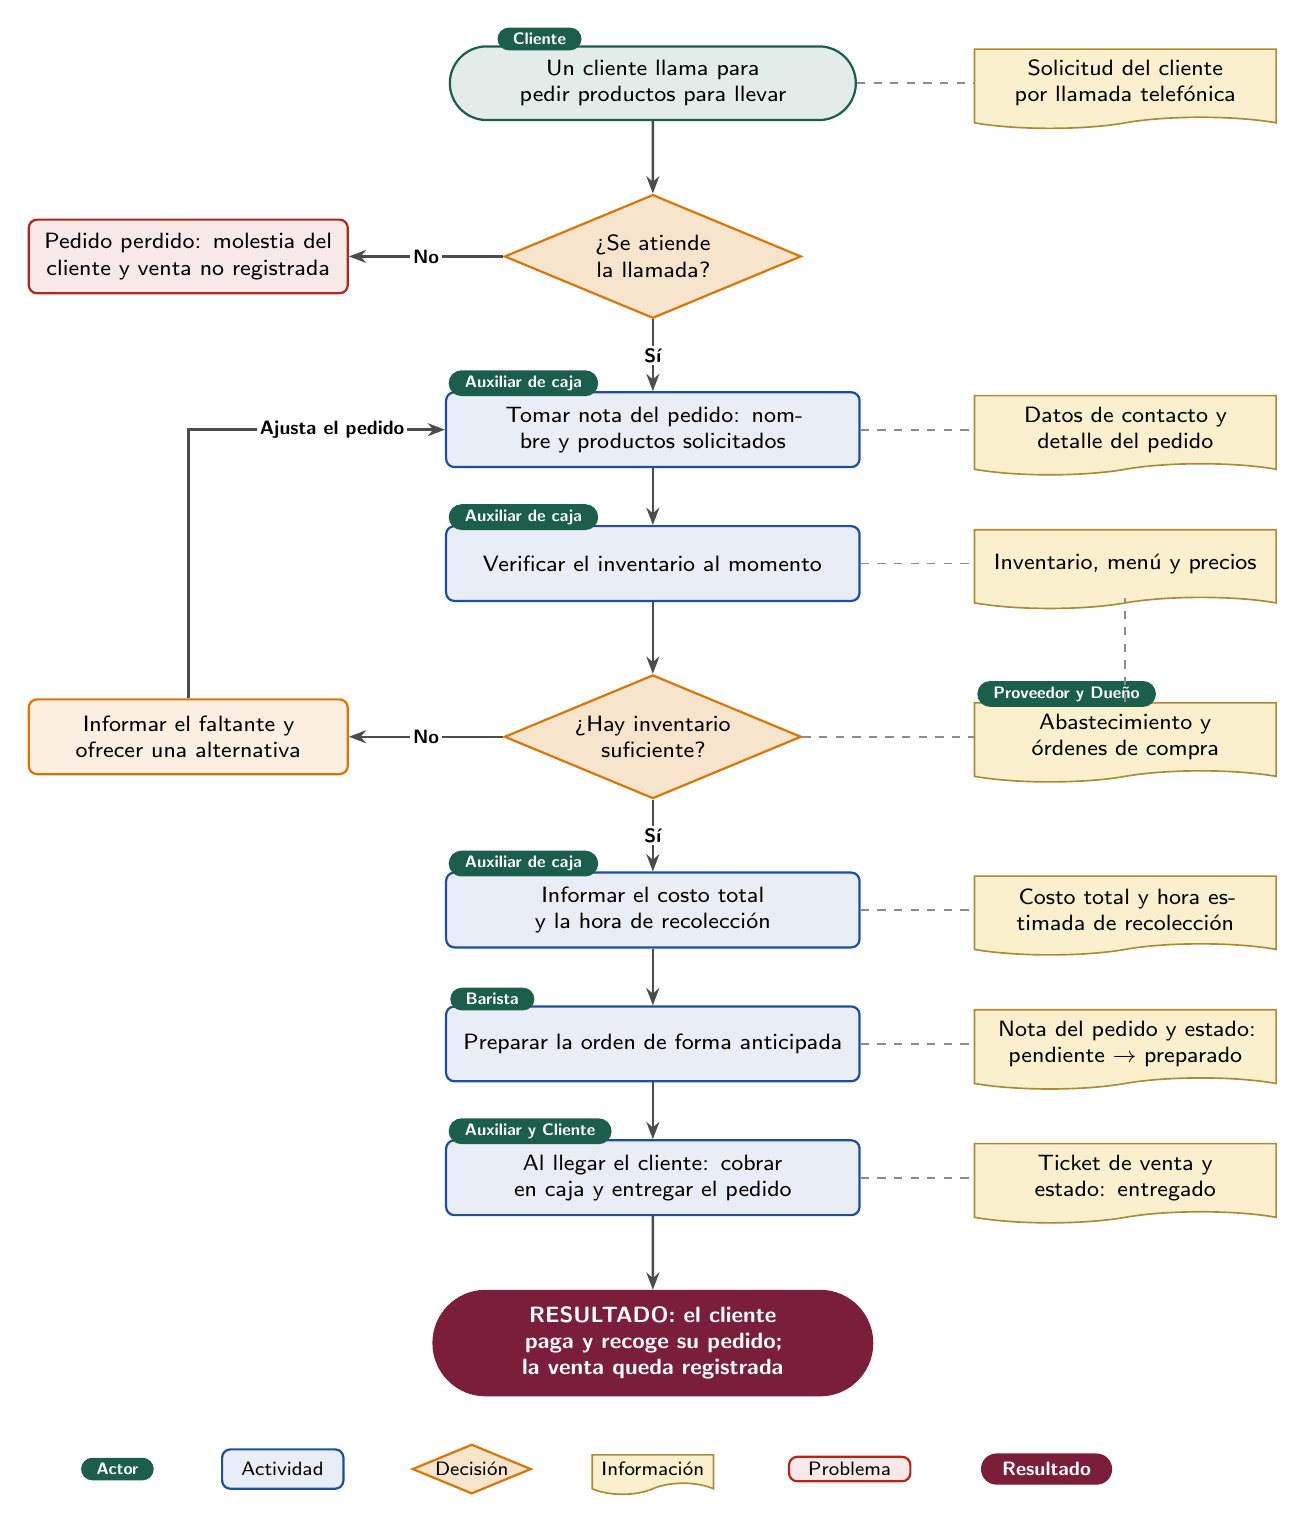
\begin{tikzpicture}[font=\sffamily\footnotesize,>={Stealth[length=2.2mm]},
act/.style={rectangle,rounded corners=3pt,draw=mazul,fill=mazul!10,line width=0.8pt,text width=4.9cm,align=center,inner sep=5pt,minimum height=0.95cm},
alterna/.style={act,draw=mnaranja,fill=mnaranja!12,text width=3.7cm},
dec/.style={diamond,aspect=2.4,draw=mnaranja,fill=mnaranja!20,line width=0.8pt,text width=2.5cm,align=center,inner sep=0pt},
ini/.style={rounded rectangle,draw=mverde,fill=mverde!12,line width=0.8pt,text width=4.6cm,align=center,inner sep=5pt},
res/.style={rounded rectangle,fill=mguinda,draw=mguinda,text=white,font=\sffamily\footnotesize\bfseries,text width=4.8cm,align=center,inner sep=6pt},
info/.style={tape,tape bend top=none,tape bend height=4pt,draw=mdorado!70!black,fill=mdorado!28,line width=0.6pt,text width=3.55cm,align=center,inner sep=4pt,minimum height=1cm},
alerta/.style={rectangle,rounded corners=3pt,draw=mrojo,fill=mrojo!10,line width=0.8pt,text width=3.7cm,align=center,inner sep=5pt},
tag/.style={rounded rectangle,fill=mverde,text=white,font=\sffamily\bfseries\fontsize{6.5}{7}\selectfont,inner xsep=5pt,inner ysep=2pt,anchor=south west},
flow/.style={->,line width=0.9pt,draw=black!70},
link/.style={dashed,draw=black!45,line width=0.6pt},
lbl/.style={font=\sffamily\bfseries\scriptsize,fill=white,inner sep=1pt}]

\node[ini] (s) at (0,0) {Un cliente llama para pedir productos para llevar};
\node[tag] at ([xshift=8pt,yshift=-2pt]s.north west) {Cliente};
\node[dec] (d1) at (0,-2.2) {¿Se atiende la llamada?};
\node[act] (n1) at (0,-4.4) {Tomar nota del pedido: nombre y productos solicitados};
\node[tag] at ([xshift=6pt,yshift=-2pt]n1.north west) {Auxiliar de caja};
\node[act] (n2) at (0,-6.1) {Verificar el inventario al momento};
\node[tag] at ([xshift=6pt,yshift=-2pt]n2.north west) {Auxiliar de caja};
\node[dec] (d2) at (0,-8.3) {¿Hay inventario suficiente?};
\node[act] (n3) at (0,-10.5) {Informar el costo total y la hora de recolección};
\node[tag] at ([xshift=6pt,yshift=-2pt]n3.north west) {Auxiliar de caja};
\node[act] (n4) at (0,-12.2) {Preparar la orden de forma anticipada};
\node[tag] at ([xshift=6pt,yshift=-2pt]n4.north west) {Barista};
\node[act] (n5) at (0,-13.9) {Al llegar el cliente: cobrar en caja y entregar el pedido};
\node[tag] at ([xshift=6pt,yshift=-2pt]n5.north west) {Auxiliar y Cliente};
\node[res] (r) at (0,-16.0) {RESULTADO: el cliente paga y recoge su pedido; la venta queda registrada};

\node[alerta] (per) at (-5.9,-2.2) {Pedido perdido: molestia del cliente y venta no registrada};
\node[alterna] (alt) at (-5.9,-8.3) {Informar el faltante y ofrecer una alternativa};

\node[info] (i0) at (6.0,0) {Solicitud del cliente por llamada telefónica};
\node[info] (i1) at (6.0,-4.4) {Datos de contacto y detalle del pedido};
\node[info] (i2) at (6.0,-6.1) {Inventario, menú y precios};
\node[info] (ip) at (6.0,-8.3) {Abastecimiento y órdenes de compra};
\node[tag] at ([xshift=6pt,yshift=-2pt]ip.north west) {Proveedor y Dueño};
\node[info] (i3) at (6.0,-10.5) {Costo total y hora estimada de recolección};
\node[info] (i4) at (6.0,-12.2) {Nota del pedido y estado: pendiente $\rightarrow$ preparado};
\node[info] (i5) at (6.0,-13.9) {Ticket de venta y estado: entregado};

\draw[flow] (s)--(d1);
\draw[flow] (d1)--(n1) node[lbl,midway] {Sí};
\draw[flow] (d1.west)--(per.east) node[lbl,midway] {No};
\draw[flow] (n1)--(n2);
\draw[flow] (n2)--(d2);
\draw[flow] (d2)--(n3) node[lbl,midway] {Sí};
\draw[flow] (d2.west)--(alt.east) node[lbl,midway] {No};
\draw[flow] (alt.north) |- (n1.west) node[lbl,pos=0.78] {Ajusta el pedido};
\draw[flow] (n3)--(n4);
\draw[flow] (n4)--(n5);
\draw[flow] (n5)--(r);

\draw[link] (s.east)--(i0.west);
\draw[link] (n1.east)--(i1.west);
\draw[link] (n2.east)--(i2.west);
\draw[link] (d2.east)--(ip.west);
\draw[link] (ip.north)--(i2.south);
\draw[link] (n3.east)--(i3.west);
\draw[link] (n4.east)--(i4.west);
\draw[link] (n5.east)--(i5.west);

\node[tag,anchor=center] at (-6.8,-17.6) {Actor};
\node[act,text width=1.4cm,minimum height=0.5cm,inner sep=2pt,font=\sffamily\scriptsize] at (-4.7,-17.6) {Actividad};
\node[dec,text width=1.1cm,font=\sffamily\scriptsize] at (-2.3,-17.6) {Decisión};
\node[info,text width=1.4cm,minimum height=0.5cm,inner sep=2pt,font=\sffamily\scriptsize] at (0,-17.6) {Información};
\node[alerta,text width=1.4cm,inner sep=2pt,font=\sffamily\scriptsize] at (2.5,-17.6) {Problema};
\node[res,text width=1.4cm,inner sep=3pt,font=\sffamily\scriptsize\bfseries] at (5,-17.6) {Resultado};
\end{tikzpicture}
}
\caption{Mapa conceptual del proceso de gestión de pedido telefónico para llevar.}
\end{figure}

\clearpage
\section{Análisis crítico individual}

\subsection{Jonathan Salinas González}
\noindent\negr{1.}\ ¿Qué riesgos existirían si una organización desarrolla software sin comprender antes sus procesos?\\
Al analizar el proceso de la Cafetería Spume Coral, pude darme cuenta de que antes de desarrollar un software es necesario conocer cómo funciona realmente una organización. Considero que muchas veces se puede pensar directamente en qué programa o sistema se podría crear para solucionar un problema, pero si no se conoce el proceso que realizan las personas involucradas, existe el riesgo de desarrollar una solución que no se adapte a sus necesidades, quedando cortos de recursos o provocando un desperdicio de tales. Uno de los principales riesgos de desarrollar software sin comprender primero los procesos es que el sistema puede resolver un problema de manera incorrecta o incluso generar nuevos problemas que inicialmente no tenías contemplados por lógica. Por ejemplo, en Cafetería Spume Coral se puede identificar que algunas llamadas de clientes que quieran realizar pedidos para llevar no necesariamente serán atendidas de manera automática por el personal el cual podía encontrarse ocupado con otras actividades. Si desarrolláramos un sistema solamente pensando en ``recibir llamadas'' sin analizar qué sucede después, podríamos crear una herramienta incompleta, que no dé seguimiento a lo que importa. Por eso considero importante primero desarmar las capas que puede llevar el proceso para no dejar que nada pase por alto.

\vspace{0.4cm}
\noindent\negr{2.}\ ¿Por qué dos organizaciones del mismo sector podrían necesitar soluciones de software diferentes?\\
Considero que dos organizaciones que pertenecen al mismo sector pueden necesitar soluciones de software diferentes porque no necesariamente trabajan de la misma manera. Dos cafeterías pueden vender productos similares, pero tener diferencias en elementos como: cantidades de empleados, formas de atender a sus clientes, horarios, proveedores o canales de venta. En el caso de Spume Coral, el problema que identificamos está relacionado principalmente con los pedidos para llevar realizados por teléfono. Por esta razón, pienso que no sería correcto asumir que una solución utilizada por una cafetería funcionará exactamente igual para otra. El software debe considerar los procesos y necesidades particulares de cada organización, por eso es importante realizar el procedimiento adecuado previo a la realización del software.

\vspace{0.4cm}
\noindent\negr{3.}\ ¿Qué información consideras crítica para modelar correctamente un proceso de negocio?\\
Para modelar correctamente un proceso de negocio considero que es crítica la información sobre los actores que participan, las actividades que realiza cada uno, la información que reciben y cómo la procesan, así como el orden en que se realizan las actividades, y en cuanto al proceso es importante revisar el flujo de sus actividades y lo que respecta las situaciones que lo pueden modificar. En nuestro caso, fue importante identificar al dueño, auxiliar de caja, barista, cliente y proveedor ya que si alguno de estos elementos no se toma en cuenta, el modelo podría representar solamente una parte del proceso y no su funcionamiento completo.

\vspace{0.4cm}
\noindent\negr{4.}\ Después de analizar el proceso de tu organización, ¿qué aspecto consideras más difícil de representar correctamente y por qué?\\
Después de analizar el proceso de la cafetería, considero que lo más difícil de representar correctamente son las situaciones que ocurren fuera de un flujo que parezca normal y simple. Porque es correcto exteriorizar y facilitar el proceso de manera abstracta, sin embargo, en la realidad pueden pasar diferentes situaciones, inclusive algunas al mismo tiempo. En este caso es importante saber cómo procesar los datos y los actores, sus roles y jerarquías para saber qué ocupación tienen en cada momento. En definitiva, las observaciones abordadas son importantes porque precisamente pueden ser causas de problemas que queremos solucionar a través del software que queremos implementar. Quiero recalcar que es indispensable el análisis de procesos de cada actor para poder construir todo, para cuando llegue el momento no tambalee el software en una situación fuera del flujo esperado o normal; en este caso, comprender el proceso de los pedidos para llevar nos permitirá identificar dónde ocurre un problema y qué características debería tener una posible solución.

\clearpage
\subsection{Keith Noelia Gómez Jose}
\noindent\negr{1.}\ ¿Qué riesgos existirían si una organización desarrolla software sin comprender antes sus procesos?\\
Si una organización ya sea una empresa grande o un negocio pequeño no analizan y comprenden los procesos que se tienen dentro es bastante probable que las decisiones y procesos no tengan un objetivo fijo al cual llegar, y, si lo tienen, no se tomarían en cuenta las opciones correctas para dicha decisión por lo cual no se llegaría a un resultado o se gastarían mas recursos teniendo perdidas de dinero y tiempo, además de darle un servicio de baja calidad a los clientes. Por estas razones es indispensable plantear y conocer muy bien los procesos que se manejan para hallar el mejor flujo hacia el resultado y poder crear un software que de verdad le sirva al negocio y mejore la experiencia del cliente.

\vspace{0.4cm}
\noindent\negr{2.}\ ¿Por qué dos organizaciones del mismo sector podrían necesitar soluciones de software diferentes?\\
Esto pasaría porque las partes que constituyen a dichas empresas tienen objetivos y alineamientos diferentes por lo que al momento de crear sus procesos estos varían puede ser desde añadir mas opciones para el cliente o tener más o menos empleados que puedan realizar una actividad para resolver las soluciones además de características como capacidad o diferentes ofertas que varían entre ellos, también son diferentes por el modelo de negocios que cada uno tiene.

\vspace{0.4cm}
\noindent\negr{3.}\ ¿Qué información consideras crítica para modelar correctamente un proceso de negocio?\\
Según lo visto en esta actividad cierta información fundamental seria conocer los actores que participan en el proceso, las actividades que cada uno de ellos desempeña, las opciones y decisiones que se toman a lo largo del desarrollo, la información que se utiliza para la realización de la actividad y la información que se entregara, y muy importante también es fijar y saber concretamente a que objetivo o resultado se quiere llegar con la realización de cada proceso, también considero importante saber el tiempo, la capacidad de operación desde el personal hasta de la infraestructura que se tiene ya que conociendo eso se pueden tomar mejores decisiones.

\vspace{0.4cm}
\noindent\negr{4.}\ Después de analizar el proceso de tu organización, ¿qué aspecto consideras más difícil de representar correctamente y por qué?\\
Un proceso que considero seria complicado de representar podría ser el abastecimiento de los ingredientes y postres ¿Por qué? Porque no siempre se utilizara la misma cantidad de ingredientes a veces sobrara mas de uno pero puede que para la siguiente vez quede mas de ese mismo ingrediente, aunque creo que esto se arreglaría con un manejo correcto en la gestión y organización de los materiales e ingredientes.

\clearpage
\subsection{Daniel Vazquez Leon}
\noindent\negr{1.}\ ¿Qué riesgos existirían si una organización desarrolla software sin comprender antes sus procesos?\\
Iniciar el desarrollo de una solución sin un mapeo exhaustivo de la lógica operativa conduce inevitablemente a la construcción de sistemas rígidos o con arquitecturas de datos inconsistentes. Si en la Cafetería Spume Coral procedemos a codificar un módulo de recepción de pedidos basándonos únicamente en la premisa de "registrar llamadas", corremos el riesgo de ignorar el ciclo de vida completo de la información. El software resultante podría generar cuellos de botella transaccionales; por ejemplo, permitiendo el ingreso masivo de órdenes sin una validación en tiempo real de los insumos disponibles. Esto no solo crearía inconsistencias en la base de datos del inventario, sino que obligaría al personal a realizar anulaciones manuales, entorpeciendo la eficiencia en lugar de optimizarla. Según los principios fundamentales de la ingeniería de requisitos, la falta de comprensión del entorno operativo resulta en soluciones que el usuario final terminará abandonando al no alinearse con su realidad.

\vspace{0.4cm}
\noindent\negr{2.}\ ¿Por qué dos organizaciones del mismo sector podrían necesitar soluciones de software diferentes?\\
Aunque dos entidades operen en la misma industria, sus reglas de negocio y restricciones operativas dictan requerimientos sistémicos diametralmente opuestos. Tomando como referencia a Spume Coral frente a otra cafetería de la región, la diferencia podría radicar en la concurrencia de sus canales de entrada o en la latencia permitida para la preparación. Mientras un establecimiento podría requerir un sistema robusto para el manejo de mesas y trazabilidad de comandas internas, en nuestro caso el volumen crítico de fallos se concentra en la asincronía de los pedidos telefónicos para llevar. Por lo tanto, nuestra solución debe priorizar interfaces de captura rápida, gestión de estados de entrega (pendiente, preparado, entregado) y alertas de tiempo límite, características que serían irrelevantes o incluso un estorbo para una organización con un modelo centrado exclusivamente en el consumo in situ.

\vspace{0.4cm}
\noindent\negr{3.}\ ¿Qué información consideras crítica para modelar correctamente un proceso de negocio?\\
Para estructurar un modelo verdaderamente funcional, considero indispensable identificar las entidades principales y el flujo de los datos a través del sistema. No basta con saber qué se hace, sino qué información detona cada evento y cómo mutan los estados de dicha información. Es crítico mapear las entradas (como los parámetros del pedido del cliente), los procesos de validación (la consulta a la base de datos de inventario) y las salidas (el ticket o la notificación de estatus). Además, resulta vital definir los roles y permisos de cada actor interactuante —el auxiliar de caja como emisor de datos y el barista como receptor y actualizador de estados— para establecer un control de concurrencia adecuado y evitar que dos procesos intenten modificar el mismo registro simultáneamente, garantizando así la integridad referencial y operativa del modelo.

\vspace{0.4cm}
\noindent\negr{4.}\ Después de analizar el proceso de tu organización, ¿qué aspecto consideras más difícil de representar correctamente y por qué?\\
Tras evaluar la dinámica de nuestra organización, concluyo que el mayor desafío analítico reside en la captura de eventos asíncronos y el manejo de excepciones operativas. Representar el "camino feliz", donde un pedido se solicita, se prepara y se cobra de manera lineal, es trivial. Sin embargo, la complejidad arquitectónica surge al intentar modelar las interrupciones del flujo principal: caídas en la comunicación, pedidos modificados en tiempo real mientras ya están en la cola de preparación, o la concurrencia de una llamada telefónica entrante justo en el momento de procesar un pago físico en caja. Determinar cómo el sistema debe priorizar, encolar o abortar estas transacciones sin perder la persistencia de los datos ya capturados, y plasmar esto en un esquema estático, requiere un nivel de abstracción alto para asegurar que el futuro software posea la tolerancia a fallos necesaria para el entorno real.

\clearpage
\subsection{Nora Lizette Mendoza Reyes}
\noindent\negr{1.}\ ¿Qué riesgos existirían si una organización desarrolla software sin comprender antes sus procesos?\\
Desde mi punto de vista, desarrollar un software sin conocer primero cómo funciona una organización puede ocasionar muchos problemas, porque se podría crear un sistema que no resuelva las necesidades reales del negocio. En el caso de la Cafetería Spume Coral, identificamos que uno de sus problemas es que algunas llamadas de clientes que desean realizar pedidos para llevar no son atendidas, debido a que los empleados se encuentran ocupados con otras actividades. Considero que, si desarrolláramos un sistema sin analizar esta situación, podríamos implementar funciones que no sean necesarias o que compliquen el trabajo de los empleados. Por eso es importante conocer primero las actividades, los actores y las decisiones que forman parte del proceso.

\vspace{0.4cm}
\noindent\negr{2.}\ ¿Por qué dos organizaciones del mismo sector podrían necesitar soluciones de software diferentes?\\
Yo considero que, aunque dos organizaciones se dediquen a la misma actividad, no necesariamente tienen los mismos problemas ni trabajan de la misma manera. Por ejemplo, una cafetería puede necesitar un sistema para controlar su inventario, mientras que otra puede necesitar uno para administrar pedidos o reservaciones. En Spume Coral, el problema que identificamos está relacionado con la atención de pedidos telefónicos. Por eso considero que una solución digital para registrar pedidos para llevar podría ser más útil que desarrollar un sistema enfocado únicamente en el inventario. Esto me permite comprender que el software debe adaptarse a las necesidades de cada organización y no al contrario.

\vspace{0.4cm}
\noindent\negr{3.}\ ¿Qué información consideras crítica para modelar correctamente un proceso de negocio?\\
Para mí, la información más importante es conocer quién realiza cada actividad, cómo comienza el proceso, qué decisiones se toman y cuál es el resultado esperado. En nuestra cafetería, necesitamos comprender cómo se recibe un pedido, quién verifica la disponibilidad de los productos, cómo se comunica la solicitud al personal encargado de prepararla y cómo se entrega al cliente. También considero importante identificar los datos que se utilizan, como los productos solicitados, las cantidades, los precios y el estado del pedido. Esta información permite representar el proceso de manera clara y detectar posibles problemas o actividades que podrían mejorarse mediante un sistema de software.

\vspace{0.4cm}
\noindent\negr{4.}\ Después de analizar el proceso de tu organización, ¿qué aspecto consideras más difícil de representar correctamente y por qué?\\
Considero que uno de los aspectos más difíciles es representar las decisiones que aparecen durante la atención de un pedido. Por ejemplo, cuando un cliente solicita un producto, primero se debe verificar si está disponible. Si no lo está, el cliente podría elegir otro producto o cancelar su pedido. También es necesario considerar qué sucede cuando un cliente intenta comunicarse por teléfono y nadie responde. Esta situación es importante porque representa el problema principal que buscamos atender. Desde mi perspectiva, estas situaciones hacen que el proceso no siempre siga un solo camino y que sea necesario analizar diferentes posibilidades.

\clearpage
\section{Relación con el proyecto integrador}

\textbf{¿Por qué se eligió esta organización?} Porque presenta un problema concreto y acotado, la pérdida de pedidos por llamadas no atendidas, que permite delimitar un proceso a analizar y plantear una solución de software viable para el Proyecto Integrador.

\textbf{¿Qué proceso es prioritario?} La recepción y atención de pedidos para llevar, especialmente cuando se solicitan por teléfono.

\textbf{¿Qué beneficios podría aportar una solución tecnológica?} Permitiría recibir solicitudes digitales, reducir la dependencia de las llamadas, ordenar los pedidos, mostrar su estado y contar con un historial para consulta. Estos beneficios son una hipótesis de trabajo que debe validarse con la cafetería, en línea con la recomendación de Pressman y Maxim (2021) de confirmar los requisitos con las partes interesadas.

\textbf{¿Qué actores serían los más afectados?} El cliente y el auxiliar de caja de manera directa; el barista y el dueño, por los cambios en la recepción, la preparación y la supervisión de los pedidos.

\section{Exposición}
El material visual utilizado para la exposición de este proyecto se encuentra disponible en el siguiente enlace:\\
\url{https://canva.link/tg7tjceeriwf3mo}

\section{Declaración obligatoria de IA}

\begin{itemize}
    \item \textbf{Herramienta utilizada:} Gemini.
    \item \textbf{Prompt principal utilizado:} ``en base a los 3 procesos que te mostré responde ¿Cómo inicia? ¿Qué actividades contiene? ¿Qué decisiones aparecen? ¿Cómo termina?''
    \item \textbf{Contenido generado por IA:} Orientación y estructuración preliminar para las respuestas de las preguntas sobre la identificación de procesos del negocio.
    \item \textbf{Contenido modificado por el equipo:} Adaptación de la información sugerida al contexto específico de la Cafetería Spume Coral, redacción de las justificaciones y elaboración completa de las reflexiones individuales garantizando la autoría del análisis crítico.
    \item \textbf{Información validada:} Los procesos, actores, variables y flujos de la cafetería fueron contrastados rigurosamente con la realidad operativa del negocio antes de su documentación y mapeo.
\end{itemize}

\section*{Referencias}
\addcontentsline{toc}{section}{Referencias}

\begin{list}{}{\setlength{\leftmargin}{1.25cm}\setlength{\itemindent}{-1.25cm}\setlength{\itemsep}{6pt}\setlength{\parsep}{0pt}}
\item Object Management Group. (2011). \textit{Business Process Model and Notation (BPMN), version 2.0}. https://www.omg.org/spec/BPMN/2.0/
\item Pressman, R. S., y Maxim, B. R. (2021). \textit{Ingeniería del software: Un enfoque práctico} (9.ª ed.). McGraw-Hill Education.
\item Sommerville, I. (2011). \textit{Ingeniería de software} (9.ª ed.). Pearson Educación.
\item Weske, M. (2019). \textit{Business process management: Concepts, languages, architectures} (3.ª ed.). Springer.
\end{list}

\end{document}